\chapter{Návrh riešenia}
V súlade so stanovenými kritériami navrhneme postupnosť krokov úpravy nameraného pohybu dopravného prostriedku. 
Zhotovenú konfigurovateľnú sústavu uplatníme na zariadení senzorovej jednotky za účelom ohlasovania udalostí 
o vybraných pravidelných rysoch signálu. Prihliadať sa bude viac na splnenie úloh v reálnom čase pri
dosiahnuteľnom výkone, v dostupnom pamäťovom priestore, ako na energetickú úsporu. Výmena údajov sa má 
odohrávať zrozumiteľným, širko podporovaným formátom, za obmedzenia nadbytočného sieťového prenosu 
v najvyššej možnej miere.


\section{Špecifikácia požiadaviek}
Zariadenie internetu vecí určené na zber a analýzu vibrácií bude realizovať nasledujúce funkčné požiadavky: 
\begin{itemize}[noitemsep,topsep=0pt]
\item Zber trojosovej akcelerácie s nastaviteľnou vzorkovacou frekvenciou a dynamickým rozsahom akcelerometra, v hraniciach danými 
obmedzeniami hardvéru, najmenej však intenzity vyskytujúcej sa pri preprave konvenčnými pozemnými motorovými vozidlami.
\item Spracovanie osí akcelerácie nezávisle s obmedzením výberu aktívnych osí.
\item Vzdialene realizovateľná zmena parametrov jednotlivých stupňov sústavy na úpravu akceleračného signálu v posuvných oknách.
\item Ukladanie nameranej akcelerácie na pamäťovú kartu s ohľadom na najvyššiu dosiahnuteľnú rýchlosť zápisu.
\item Identifikácia významných frekvencií zo vzoriek akcelerometra so zachytením ich trvania a amplitúdy podľa aktuálnej 
konfigurácie detekčných algoritmov.
\item Sumarizácia hodnôt akcelerácie po posuvných oknách do popisných štatistík.
\item Odosielanie zachytených udalostí cez spoľahlivé sieťové spojenie za dosiahnutia redukcie množstva dát oproti priamo odčítaným vzorkám. 
\item Poskytnutie možnosti odosielania výstupov z podstatných medzikrokov spracovania za účelom potenciálneho ponechania 
analýzy pre ďalšie úrovne senzorovej siete alebo skupinovej koordinácie údajov z viacerých uzlov. 
\end{itemize}
\bigskip

Z povahy okolností nasadenia firmvéru na relatívne zdrojovo oklieštené Edge zariadenie vyplývajú 
vymenované nie-funkčné požiadavky, prevažne na účinnosť a prenositeľnosť:
\begin{itemize}[noitemsep,topsep=0pt]
\item Firmvér sa zmestí do programovej pamäte s rezervou pre budúce rozširovanie funkcionality.
\item Ľubovoľný scenár spracovania musí prebehnúť v reálnom čase.
\item Odozva detekcie udalostí bude najkratšia možná.
\item Výmena údajov cez sieťové protokol v štandardizovanom formáte hierarchickej štruktúry za najmenšej uskutočniteľnej réžie.
\item Platformová závislosť sa obmedzí na nevyhnuté súčasti systému ako sú hardvérové ovládače a akcelerácia náročných výpočtov.
\end{itemize}

\section{Hardvér senzorovej jednotky}
Navrhované zariadenie bude postavené na mikrokontroléri ESP32 od Espressif, pretože pri nízkej obstarávacej cene
ponúka možnosť konektivity na 2,4 GHz s Wifi 802.11 b/g/n a Bluetooth 4.2. V porovnaní s podobnými zariadeniami disponuje 
nebývalým výpočtovým výkonom a kapacitou pamätí.

Konkrétne zvolíme dosku FireBeetle osadenú modulom \emph{ESP32-WROOM-32D} s typickým napájacím napätím 3,3 V a dvoj-jadrovým 
32-bitovým procesorom Xtensa s taktovacou frekvenciou od 80 do 240 MHz. Modul obsahuje až 520 kB zdieľanej SRAM 
pre inštrukcie a dáta. 

Použitý model akcelerometera je súčasťou MEMS inerciálnej meracej jednotky \emph{LSM9DS1} zabudovanej na doske
STEVAL-MKI159V1 slúžiacej na adaptáciu pre púzdro DIL24. Akcelerometer bude s mikrokontrolérom komunikovať cez
poloduplexnú SPI zbernicu s horným obmedzením frekvencie hodín na 8 MHz. Navyše budú zapojené aj vývody prerušení INT1 a INT2
pre upozornenie prekročenia určených prahových úrovní. Blokový diagram zapojenia je na schéme na obr. \ref{schematics:block}.

\begin{figure}[h]
\centering
\begin{subfigure}[b]{0.65\textwidth}
    \centering
    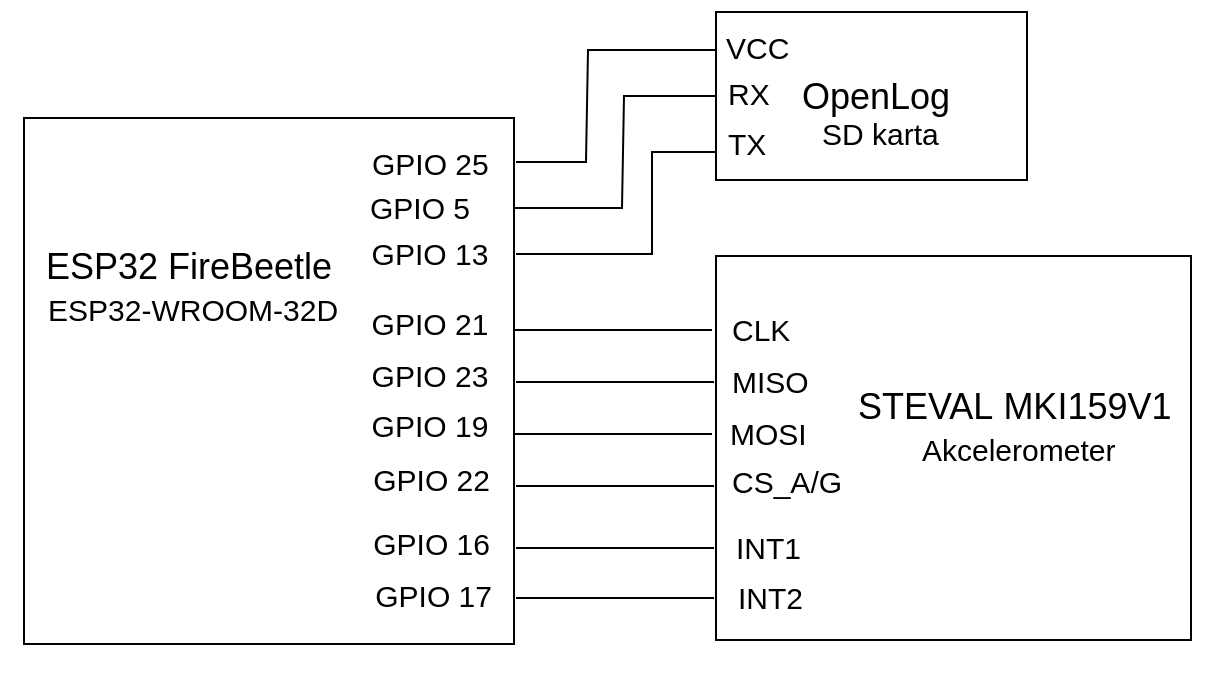
\includegraphics[width=\textwidth]{figures/design/block-circuit-diagram.png}
    \caption{Blokový diagram modulov}
       \label{schematics:block}
\end{subfigure}
\hfill
\begin{subfigure}[b]{0.3\textwidth}
    \centering
    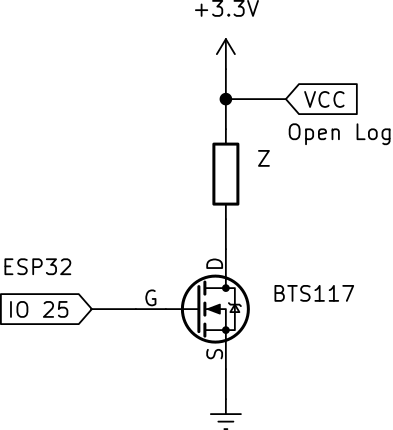
\includegraphics[width=\textwidth]{figures/design/fet.png}
    \caption{Ovládanie napájania OpenLog cez FET}
    \label{schematics:fet}
\end{subfigure}
\label{schematics}
\caption{Schéma zapojenia hardvéru}
\end{figure}
 
Pamäťová Micro SD karta so súborovým systémom FAT32 bude pripojená v module \emph{OpenLog} od Sparkfun, ktorý zaznamená znakový
vstup prijímaný UART zbernicou do  textových súborov podľa pravidiel zo súboru \verb|config.txt| alebo povelmi odoslaných 
po zapnutí. Ukladať vzorky na externé médium nie je vždy žiaduce, preto bude napájanie spínané cez pin mikrokontroléra. Vyšší 
prúdový odber než dodá výstup a požadované napätie rovné s napájacím napätím dosky vyžaduje umiestnenie tranzistora riadeného 
poľom N-kanál \emph{BTS117} na premostenie riadiaceho signálu podľa obr. \ref{schematics:fet}.


\section{Architektúra systému}
Celková skladba komponentov systému pozostáva zo súčastí pôsobiacich na mikrokontroléri ESP32
interagujúcimi s akcelerometrom a zapisovačom cez lokálne sériové zbernice. Výstupy uspôsobenia a zoskupenia vektorov akcelerácie sú 
odosielané do počítačovej siete prostredníctvom prístupového bodu WiFi aplikačným protokolom MQTT (Message Queue Transport Telemetry)
na server poskytujúci službu MQTT broker správ Eclipse Mosquitto. Odtiaľ sú odoberané témy prešírené klientom metódou publish -- subcribe.
Diagram na obr. \ref{uml:component} zachytáva náhľad na poskladanie komponentov systému. 

\begin{figure}[h]
	\centering
	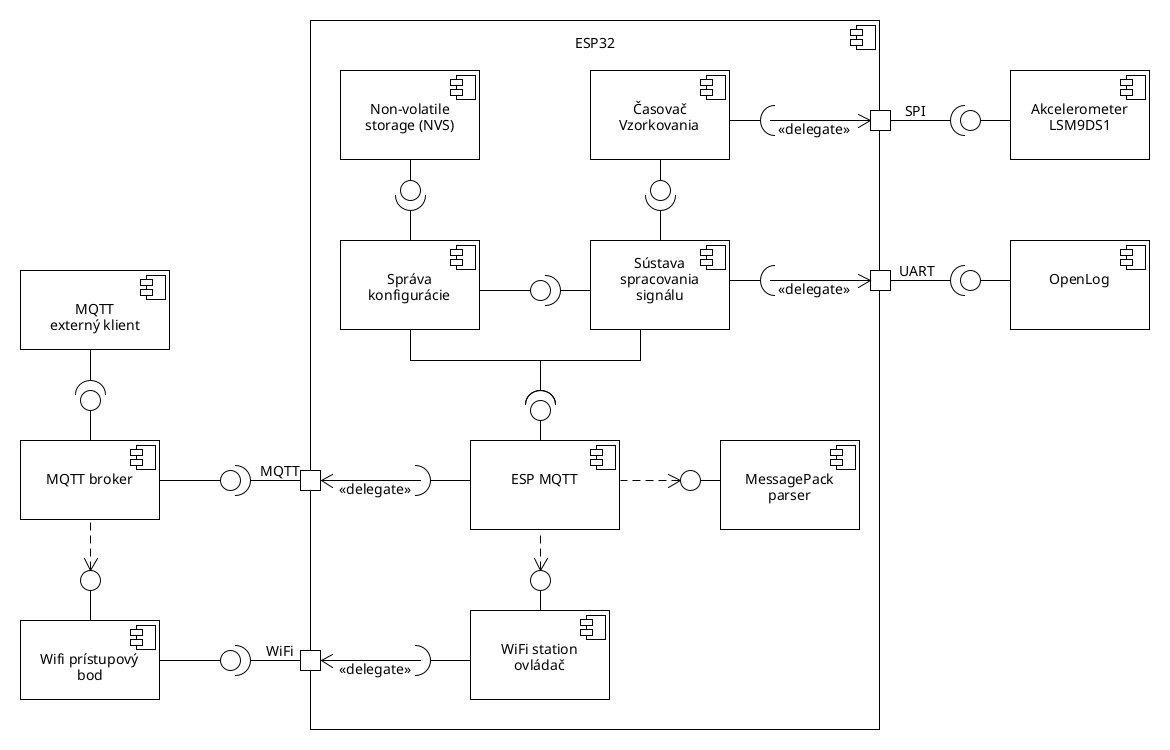
\includegraphics[width=\textwidth]{figures/design/components.png}
	\caption{Diagram komponentov}
	\label{uml:component}
\end{figure}

Odčítavanie úrovní z akcelerometra zabezpečuje časovač vzorkovania, ktorý si v pravidelných intervaloch pýta aktuálne hodnoty rozhraním 
periférneho adaptéra pre prístup ku SPI zbernici. Po vypršaní vzorkovacej periódy je zavolaná obsluha prerušenia, ktorá odblokuje vlákno 
úlohy na synchrónne načítanie okamžitého vektora zrýchlenia konvertovaného z číslicovej úrovne prevodníka na SI jednotku $m/s^2$. 
Postup vzorkovania ilustruje sekvenčný diagram na obr. \ref{uml:sequence}.

Zachytené hodnoty sú preposlané do nezávislých thread-safe front analyzátora signálu pre individuálne priestorové osi akcelerácie. 
V prípade nutnosti zachytávať ucelený priebeh veličiny  sa vektor umiestni do frontu ku vláknu loggera. Postup vzorkovania 
ilustruje sekvenčný diagram na obr. \ref{uml:sequence}. Pipeline spracovania signálu rozdeľuje vzorky do prelínajúcich sa posuvných okien, 
počíta z nich štatistiky a vyhľadáva udalosti vo frekvenčnom spektre. Nespracované hodnoty sú podľa potreby ukladané na pamäťovú kartu. 

Zmenu a uchovanie parametrov pipelinov pre jednotlivé bloky spracovania zaobstaráva správa konfigurácie. Modifikované nastavenia sú medzi 
spusteniami zachované vo vyhradenej partícií nevolatilnej flash pamäte na záznamy dvojíc v asociatívnej štruktúre. Predvolené správanie 
načítané pre nedostupnosť stavu z flash úložiska určujú konštanty v programovej pamäti.

Binárny serializačný formát Message Pack zaobaluje vzorky, udalosti a konfigurácia posielané na rozličné MQTT témy. Vychádza z 
formátu JSON (JavaScript Object Notation), ale narozdiel od neho sa sústredí na efektívne kódovanie dátových typov. Namiesto prevodu 
číselných údajov do znakového kódovania, napr. Unicode, ponecháva ich pôvodnú binárnu reprezentáciu s špecifikovanou bytovou značkou 
určujúcou typ. Hodnoty vyjadriteľné menším počtom bajtov reprezentuje dokonca v kratšom tvare než podmieňuje ich celkový rozsah.
Rovnako v zoznamoch a slovníkov sa  zaobchádza bez oddelovacích znakov, ktoré nahrádza informáciou o počte údajov. Dĺžka 
položky predchádzajúca zloženými atribútom uľahčuje následné parsovanie.

\begin{figure}[h]
	\centering
	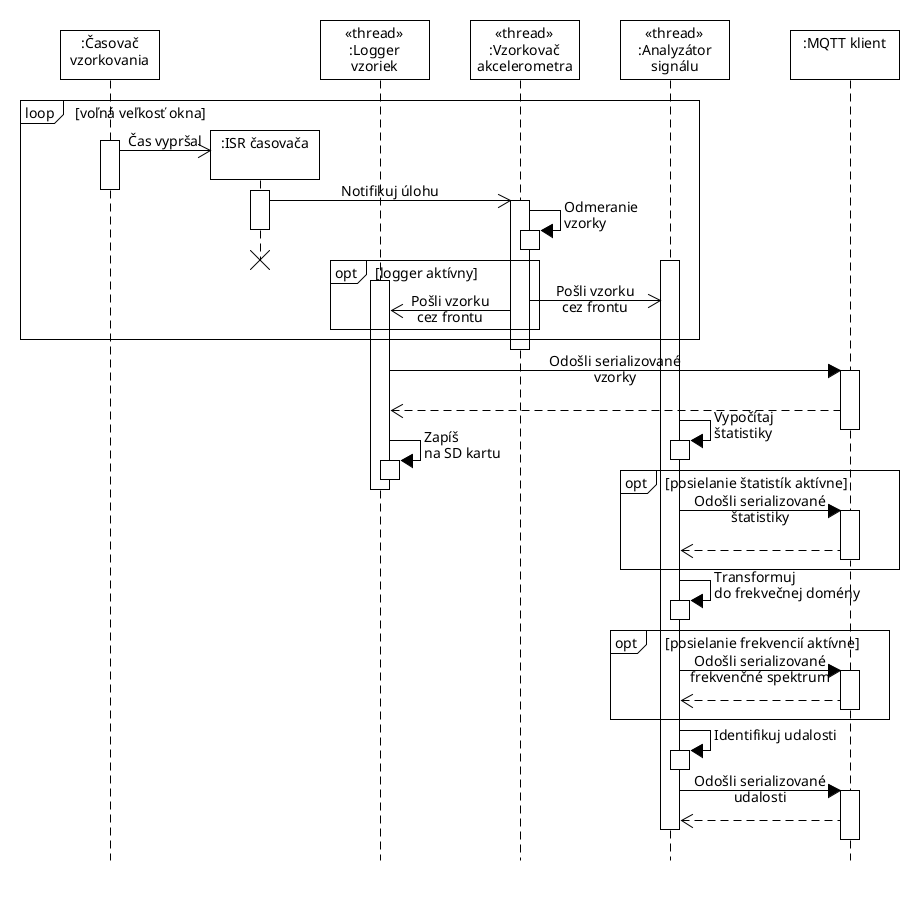
\includegraphics[width=\textwidth]{figures/design/tasks.png}
	\caption{Sekvenčný diagram vzorkovania signálu}
	\label{uml:sequence}
\end{figure}

\section{Funkčné bloky dátovej pipeline}

\begin{figure}[h]
	\centering
	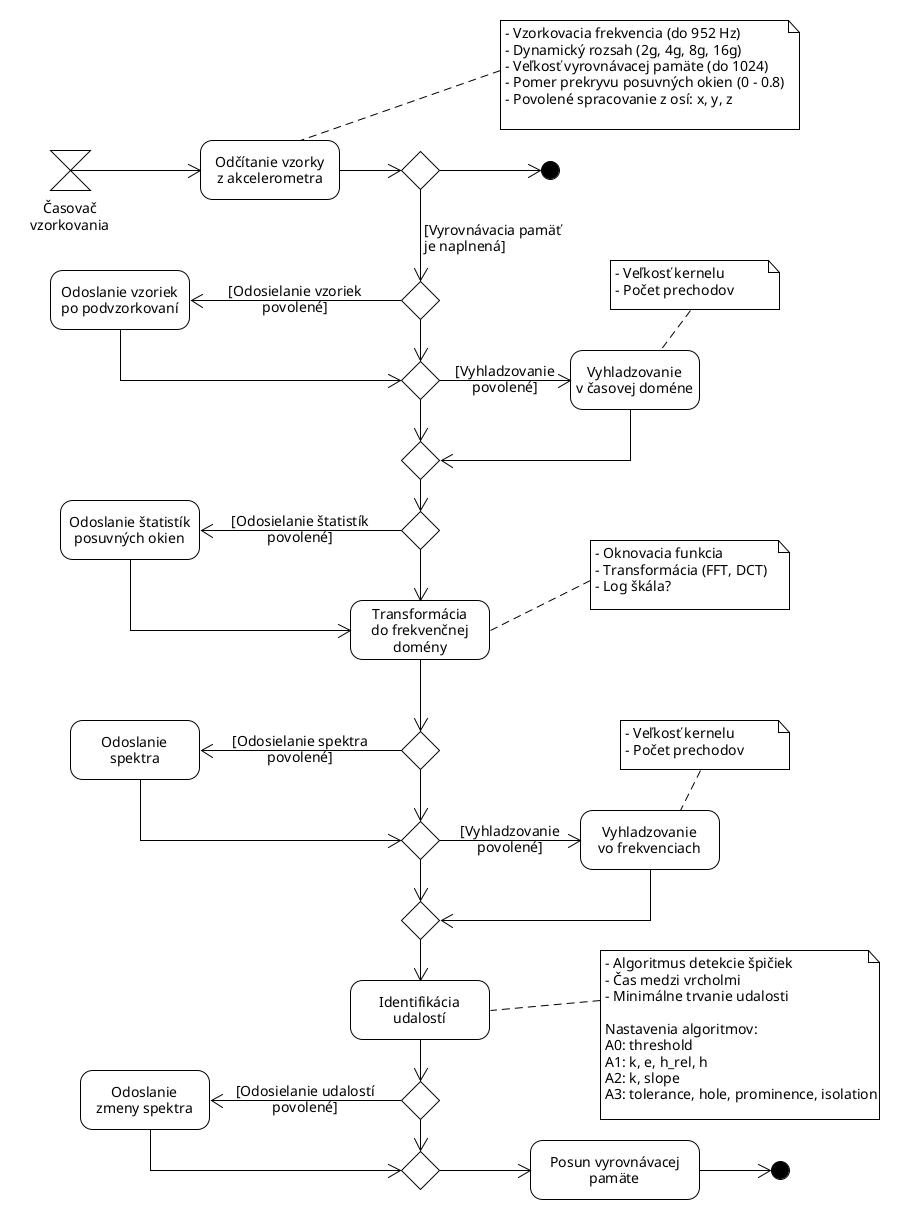
\includegraphics[width=\textwidth]{figures/design/pipeline.png}
	\caption{Diagram aktivít navrhovaného systému na spracovanie dát zo senzora}
\end{figure}


\begin{figure}[h]
	\centering
	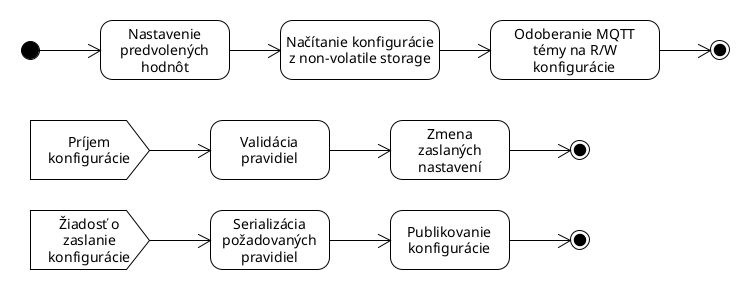
\includegraphics[width=\textwidth]{figures/design/configuration.png}
	\caption{Diagram aktivít konfigurácie}
\end{figure}

Podľa pravidlami aktivovanými modulmi bude súbežne vykonateľných 5 ciest spracovania. 
Frekvenčná analýza bude pozostávať z krokov oknovania signálu  zvoliteľnou oknovou funkciou nastaviteľnej veľkosti,
následne sa signál transformuje do frekvenčnej domény,
kde dôjde k vyhladeniu spektra kĺzavým priemerom alebo Welchovou metódou a nakoniec sa podľa prítomnosti špičiek
vo frekvenčnom vedierku vytvorí udalosť na začiatku a na konci súvislého časového pôsobenia. Časová analýza
bude detegovať náhle zmeny v priebehu signálu na základe štatistík polohy, rozptýlenosti a tvaru
distribúcie vzhľadom na predošlé okná. Okrem toho sa môžu po podvzorkovaní odosielať alebo ukladať ,,surové dáta''
hodnôt veličiny v čase alebo frekvenčných vedierok. Numerická kvadratúra korigovaná obálkami umožní extrahovať zo
snímaného zrýchlenia odhad o rýchlosti a polohe.

Diagram aktivít na obr. \ref{fig:design}
vizualizuje navrhovaný beh činností na zariadení.

\clearpage


\section{Prúdový algoritmus detekcie zmien frekvencií}
Nevidí celý prúd naraz ani ho nemôže celý uložiť. Welchove priemerovanie vyžaduje veľa pamäte pre dlhšie okno.
Ale musíme dosiahnuť odšumenie detegovanie špičiek a zároveň posielať cez sieť menej ako nespracované
frekvenčné vedierka. Detegovanie anomálií, resp. automatické upozornenie na prevládajúce zložky.

\begin{figure}[h]
\centering
\begin{subfigure}[b]{0.8\textwidth}
    \centering
    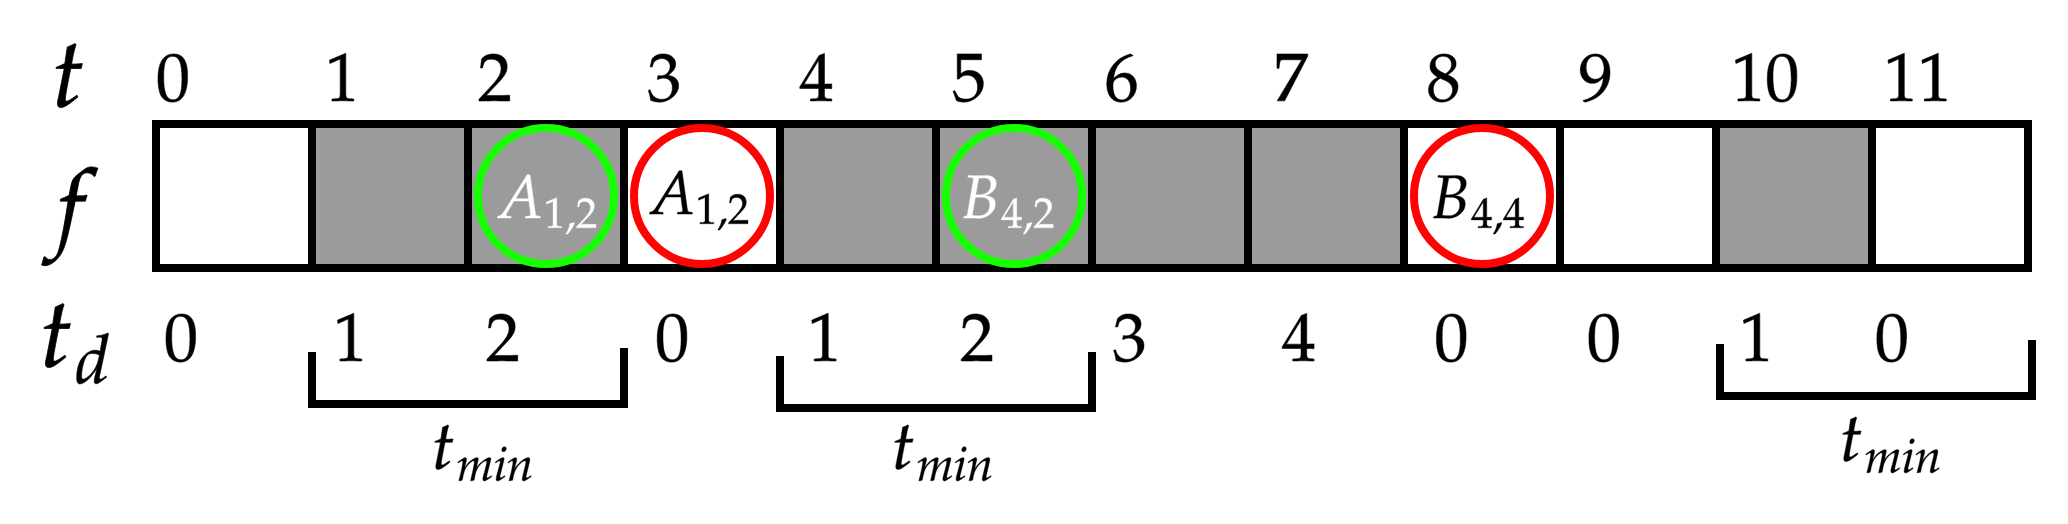
\includegraphics[width=\textwidth]{figures/design/event-detection-min-duration.png}
    \caption{Minimálne trvanie udalosti $t_{\min} = 2$}
\end{subfigure}
\begin{subfigure}[b]{0.8\textwidth}
    \centering
    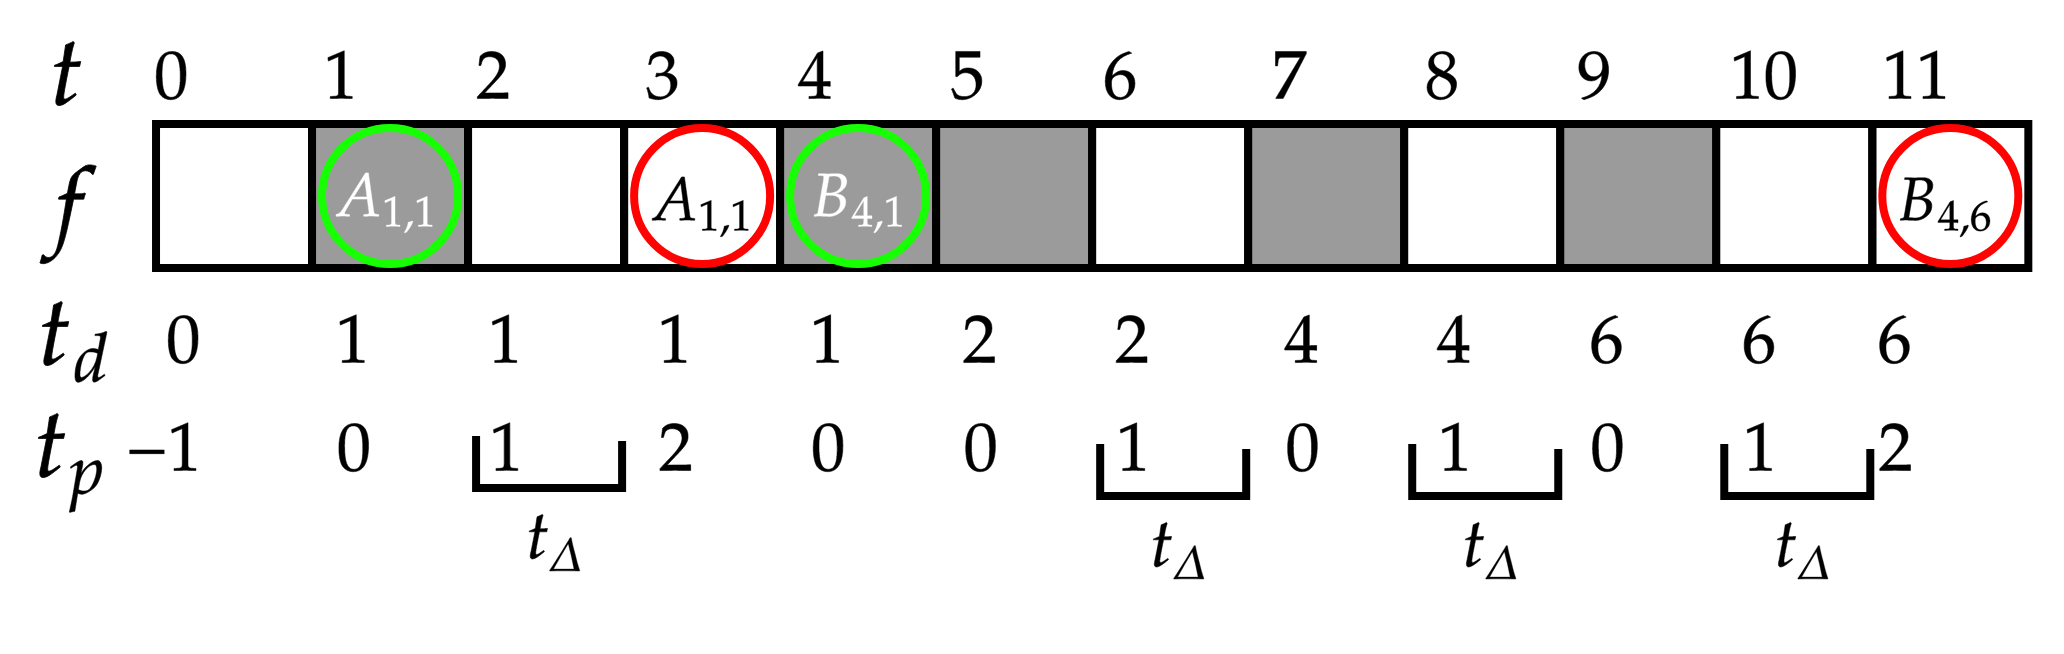
\includegraphics[width=\textwidth]{figures/design/event-detection-time-proximity.png}
    \caption{Maximálna vzdialenosť špičiek $t_{\Delta} = 1$ v čase}
\end{subfigure}
\caption{Parametre algoritmu na detekciu udalostí. $t$ je poradové číslo okna, $f$ je stav detegovanie špičky
vo frekvenčnom vedierku, $t_d$ je trvanie udalosti (duration), $t_p$ je počet okien do minulosti naposledy videnej špičky (past)}
\end{figure}

\begin{algorithm}[h]
\caption{Detektor zmeny frekvenčnej zložky}
\begin{algorithmic}[1]
\Require{$event$, $bin$, $t$, $t_{min}$, $t_{\Delta}$}
\If {V predošlom okne $t - 1$ bola emitovaná udalosť Koniec}
	\State Vynuluj udalosť: $event$: $duration \gets amplitude \gets 0$, $lastSeen \gets -1$
\EndIf

\If {$\mathrm{IsPeak}(bin)$}  
	\State $link \gets \max\{1, event.lastSeen + 1\}$
	\If {$event.duration < t_{min} \leq event.duration + link$}
		\State $event.start \gets t - event.duration - link + 1$
		\State \textbf{Emituj udalosť Štart} výskytu frekvencie podľa $event$
	\EndIf
	
	\State \textbf{Inkrementuj} $event.duration$ \textbf{o} $link$
	\State \textbf{Inkrementuj} $event.amplitude$ \textbf{o} $(bin - event.amplitude)\;/\;event.duration$
	\State $event.lastSeen \gets 0$

\ElsIf {$event.lastSeen \geq 0$}
	\State \textbf{Inkrementuj} $event.lastSeen$ \textbf{o}  $1$

	\If {$events.lastSeen > t_{\Delta}$}
        	\If {$event.duration \geq t_{min}$}
        		\State \textbf{Emituj udalosť Koniec} výskytu frekvencie podľa $event$
        	\EndIf
        \Else
        	\State Vynuluj udalosť: $event$: $duration \gets amplitude \gets 0$, $lastSeen \gets -1$
        \EndIf
\EndIf
\end{algorithmic}
\label{algo:event-detector}
\end{algorithm}

\section{Zber vibrácií z premávky}
V časti motora alebo nad nápravou z mestskej hromadnej dopravy. 500Hz, rozlíšní 2g z v režime zapisovania na SD kartu.
Predošlé prieskumné merania na akcelerometri smarfónu ukázali rozsah do +/-$8 m/s^2$do 1g najčastejšie do $2 - 3 m/s^2$

Pre LSB formát je tesne pod teoretickou hranicou rýchlosti UART (115200 baud). 1 znak = 8b + štart + stop = 10bitov.
Rozsah hodnôt signed int16 (5-ciferné číslo a znamienko na jednu súradnicu). Riadok mal teda aj s medzerami a novým riadkom max.
21 znakov na 3D vzorku. 21 znakov je 210 bitov. Teoretická max. vzorkovacia frekvencia je 548 Hz.

Realistické vzhľadom k prevážanému obsahu

\section{Generátor frekvenčného spektra}
Opis políčok konfigurácie a postup generovania fade-in/out sinsoid a náhodné vkladanie do signálu

\begin{figure}[h]
   \centering
    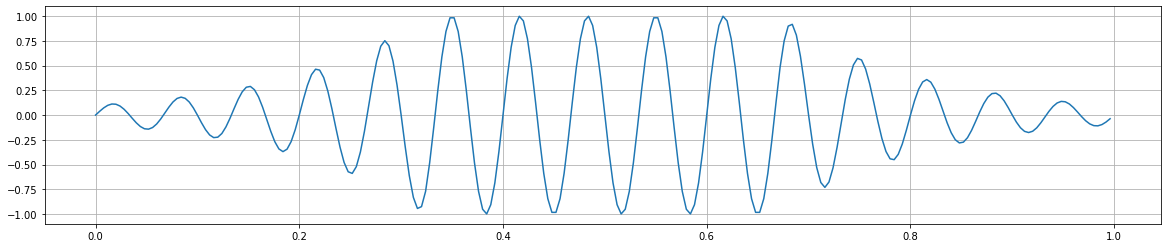
\includegraphics[width=0.8\textwidth]{figures/verification/fade-in-sinusoid.png}
   \caption{Základný tón formujúci syntetický signál}
\end{figure} 
